\documentclass[12pt,a4paper]{report}

\usepackage{titlesec}									% Formating Titles 
\usepackage{indentfirst}                              	% First line as paragraph format  
	\setlength\parindent{1cm}                              	% Spacing from left margin
	\renewcommand{\baselinestretch}{1.50}\normalsize       	% Line spacing
\usepackage{times}                                    	% Font name
\usepackage{anysize}                                  	% Setting page                    
	\marginsize{1.25in}{.75in}{1in}{1in}

\usepackage{amsmath}									% format multi-line equations
\usepackage{amsfonts}
\usepackage{graphicx}									% Figure width, height, angle,ascept ratio ....
\graphicspath{{Images/}}
\usepackage{setspace}									% Double spacing
\usepackage{fancyhdr}									% Headers & Footers
\usepackage{nomencl}									% Include List of nomenclature
\usepackage[table]{xcolor}								% Colouring inside tables
\usepackage{multirow}									% Combaining rows or columns in tables 
\usepackage{rotating}									% Rotation of figures, tables
\usepackage[hypcap]{caption}							% Captions fonts....
\usepackage{subcaption}									% Caption in minipage. (Subfigure)
\usepackage{array}										% for matrix tables etc
\usepackage{subfig}										% Subfigures (Side to side figure)

\usepackage[overload]{textcase}							% Mahing Upper Case
\usepackage{color, colortbl}							% Defines colors
\usepackage{csquotes}									% Including single quotes or double quotes
\usepackage{makeidx}									% Making Index page
\usepackage{float}										% Forcing the figures in places
\usepackage[most]{tcolorbox}							% Includes colors inside table box
\usepackage[toc,page]{appendix}							% Including Appendix
\usepackage{emptypage} 									% Making empty page in latex when starting right
\usepackage{pdfpages}									% Including PDF files

%\usepackage{chngcntr}									% Numbering as per our wish
	%%\counterwithin{figure}{section}
	%\counterwithout{figure}{chapter}
%\usepackage{listings}									% include the source code 
\usepackage{tocloft}

\usepackage{enumitem}


\titleformat{\chapter}[display]
{\normalfont\Large\bfseries\centering}
{\chaptertitlename\ \thechapter}{5pt}{\Large}
\titlespacing*{\chapter}{0pt}{-15pt}{35pt} % First: Second: From top; Third: Spacing after title
\titleformat{\section}{\large\bfseries}{\thesection}{1em}{}
\titleformat{\subsection}{\normalsize\bfseries}{\thesubsection}{1em}{}
\renewcommand{\chaptermark}[1]{\markboth{ \emph{#1}}{}}
\renewcommand{\chaptermark}[1]{\markboth{ \emph{#1}}{}}




\begin{document}

\thispagestyle{empty}
\begin{doublespace}

\begin{center}
	\textsc{\textbf{\huge{Mini Project Name}}}
\end{center}

\vspace{0.15cm}

\begin{center}
	\textsc{\textbf{\Large{Mini Project Report}}}
\end{center}

\vspace{0.1cm}

\begin{center}
	\large{\textit{Submitted in partial fulfillment of the requirements for the award of the\\ Degree of \textbf{Bachelor of Technology} in \textbf{Electronics \& Communication\\ Engineering} of \textbf{APJ Abdul Kalam Technological University}}}
\end{center}

\vspace{0.02cm}

\begin{center}
	\large{By}
\end{center}

\begin{center}
	\textsc{\textbf{\large{Your Name}}}\\
	\textsc{\textbf{\large{(VI Semester B.Tech, Reg No. MDL22xxxx)}}}
\end{center}

\begin{figure}[H]
	\begin{center}
		\leavevmode
			
\includegraphics[width=.25\textwidth]{LogoMEC}
	\end{center}
\end{figure}

\vspace{0.02cm}

\tikz[remember picture,overlay,opacity=0.25]\node[anchor=south,inner sep=0pt] at (current page.south) {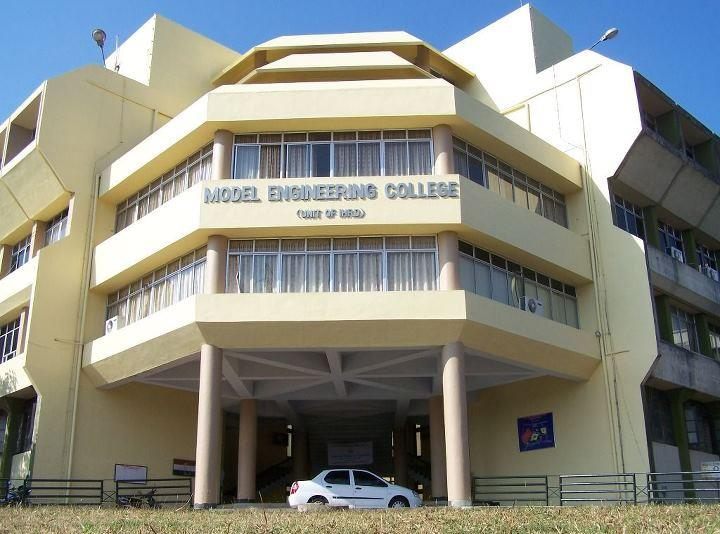
\includegraphics[width=\paperwidth]{MEC}};

\begin{center}
\textsc{\textbf{\Large{April 2025}}}
\end{center} 

\vspace{0.1cm}

\begin{center}
\textbf{\textsc{\Large{Department of Electronics Engineering}}\\
\textsc{\Large{Model Engineering College, Thrikkakara}}\\
\textsc{\Large{Ernakulam}}} 
\end{center}

\end{doublespace}
\thispagestyle{empty}
\begin{doublespace}

\begin{center}
	\textsc{\textbf{\Large{Model Engineering College, Thrikkakara}}}
\end{center}

\begin{figure}[H]
	\begin{center}
		\leavevmode
			
\includegraphics[width=.25\textwidth]{LogoMEC}
	\end{center}
\end{figure}

\vspace{0.1cm}

\begin{center}
	\textsc{\textbf{\Large{Department of Electronics Engineering}}}
\end{center}

\vspace{0.05cm}

\begin{center}
\textbf{\textit{\Large{\underline{CERTIFICATE}}}}
\end{center}


	\textit{This is to certify that the project report entitled \textsc{\textbf{\enquote{Mini Project Name}}} is a bonafide record of the project work done by \textsc{\textbf{Your Name}} (VIII Semester B.Tech, Reg No. MDL23XXX) towards the partial fulfillment of the requirements for the award of the Degree of Bachelor of Technology in Electronics \& Communication Engineering of APJ Abdul Kalam Technological University during the year 2025.}
	
\end{doublespace}	

\vspace{1cm}
\begin{minipage}[b]{0.45\linewidth}\centering
	\begin{flushleft}
		\hspace{-0.5cm}\textbf{\textsc{\normalsize{Project Co-ordinator}}}\\
		\vspace{1cm}
		\hspace{-0.5cm}\textbf{\textsc{\small{Coordinator Name}}}\\
		\hspace{-0.5cm}\textsc{\small{Designation}}\\
		\hspace{-0.5cm}\textsc{\small{Dept. of Electronics}}
	\end{flushleft}
\end{minipage}
\hspace{0.5cm}
\begin{minipage}[b]{0.45\linewidth}
	\begin{flushright}
		\textbf{\textsc{\normalsize{Project Guide}}}\\
		\vspace{1cm}
		\textbf{\textsc{\small{Guide Name}}}\\
		\textsc{\small{Designation}}\\
		\textsc{\small{Dept. of Electronics}}
	\end{flushright}
\end{minipage}
\begin{center}
\textbf{\textsc{\normalsize{Head of Department}}}\\
\vspace{1cm}
\textbf{\textsc{\small{HoD Name}}}\\
\textsc{\small{Dept. of Electronics Engineering}}
\end{center}


\thispagestyle{empty}
\makenomenclature
\renewcommand{\nomname}{List of Abbreviations}


\newpage
\pagenumbering{roman}

\newpage
\section*{\begin{center} \Large{ACKNOWLEDGEMENT}\end{center}}
{\textit{First of all, I would like to thank the \textbf{Lord Almighty} who helped me to finish this project on time.}

\textit{I express my sincere thanks to \textbf{}, The Principal, Model Engineering College, Thrikkakara, for providing opportunity and the environment to do the project in my college.}

\textit{I sincerely thank \textbf{}, Head of the Department, Dept. of Electronics, for his encouragement and constant support in making project successful.}

\textit{I would like to thank my class coordinator \textbf{M. } , Asst. Professor, Dept. of Electronics, for giving me timely instruction,for the completion the work.}

\textit{I would like to thank my project coordinator \textbf{M. } , Asst. Professor, Dept. of Electronics, for giving me technical advice, without which I could never been able to complete the work in time.}

\textit{I also wish to thank my project guide \textbf{M. }, Asst. Professor, Dept. of Electronics, for providing valuable guidance.}

\textit{An excellent group of teaching and non-teaching staff helped me for this project. I owe much the assistance they gave me while doing the project.}

\textit{Last, but not least I would like to thank my parents and friends for all the moral support and that they have given me.}


\begin{flushright}
Your Name \hspace{.2cm} (Roll No.)
\end{flushright}
}




\newpage
\section*{\begin{center} \Large{ABSTRACT}\end{center}}
\thispagestyle{plain}
\par
{
Lorem ipsum dolor sit amet, consectetur adipiscing elit. Curabitur non velit leo. Nullam dapibus libero condimentum tellus vehicula suscipit. Mauris non finibus augue. Nunc urna tellus, dapibus eu tellus ac, hendrerit pretium quam. Mauris dapibus nec ante nec iaculis. Mauris sodales felis sed neque volutpat venenatis. Morbi pellentesque sit amet dolor a rhoncus. Phasellus interdum augue quis dui vehicula malesuada. Quisque nisl dolor, ornare quis sodales vel, fermentum nec neque. 
}



\clearpage
\begin{doublespace}
\renewcommand{\contentsname}{\begin{center} \Large \textbf{Contents} \end{center}}
\tableofcontents            % print the table of contents
\end{doublespace}

        		% print list of figures
\clearpage
\renewcommand{\listfigurename}{\begin{center} \Large \textbf{List of Figures} \end{center}}
\renewcommand{\cftfigfont}{Fig. }
\addcontentsline{toc}{section}{List of Figures}
\listoffigures

				% print list of tables
\clearpage
\renewcommand{\listtablename}{\begin{center} \Large \textbf{List of Tables} \end{center}}
\renewcommand{\cftfigfont}{Table: }
\addcontentsline{toc}{section}{List of Tables}
\listoftables

 
\printnomenclature[2.5cm]

\addcontentsline{toc}{section}{List of Abbreviations}

% Generates a list of Abbreviations
% Type the acronys and expansions below

\newlist{abbrv}{itemize}{1}
\setlist[abbrv,1]{label=,labelwidth=1in,align=parleft,itemsep=0.1\baselineskip,leftmargin=!}

\chapter*{List of Abbreviations}
\chaptermark{List of Abbreviations}

\begin{abbrv}

\item[EC ]			Electronics and Communication
\item[EV ]			Electronics and VLSI
\item[EE ]			Electrical and Electronics 
\end{abbrv}

%\addtocontents{file}{text}

\newpage
\pagestyle{fancy}
\headheight 26pt
\renewcommand{\footrulewidth}{1.2pt}
\renewcommand{\headrulewidth}{1.2pt}
\rhead[OC]{\rmfamily \small \nouppercase \leftmark}
%\chead{Middle top}
\lhead{\small{Mini Project, 2025}}
\rfoot{\small{Model Engineering College, Thrikkakara}}
\cfoot{\thepage}
\lfoot{\small{Department of Electronics Engineering}}


\fancypagestyle{plain}
\newpage
\pagenumbering{arabic}


\newpage
\pagenumbering{arabic}

\chapter{INTRODUCTION}
\thispagestyle{empty}
Lorem ipsum dolor sit amet, consectetur adipiscing elit, sed do eiusmod tempor incididunt ut labore et dolore magna aliqua. Ut enim ad minim veniam, quis nostrud exercitation ullamco laboris nisi ut aliquip ex ea commodo consequat.\cite{JSM}\nomenclature[Ch]{Ch}{Chapter} 


\section{Background of the Project}
Lorem ipsum dolor sit amet, consectetur adipiscing elit. Curabitur non velit leo. Nullam dapibus libero condimentum tellus vehicula suscipit. Mauris non finibus augue. Nunc urna tellus, dapibus eu tellus ac, hendrerit pretium quam. Mauris dapibus nec ante nec iaculis. Mauris sodales felis sed neque volutpat venenatis. Morbi pellentesque sit amet dolor a rhoncus. Phasellus interdum augue quis dui vehicula malesuada. Quisque nisl dolor, ornare quis sodales vel, fermentum nec neque. \cite{HAR}

\begin{enumerate}
\item First point.
\item Second point.
\end{enumerate}

\subsection{Subsection Name}
Lorem ipsum dolor sit amet, consectetur adipiscing elit. Curabitur non velit leo. Nullam dapibus libero condimentum tellus vehicula suscipit. Mauris non finibus augue. Nunc urna tellus, dapibus eu tellus ac, hendrerit pretium quam. Mauris dapibus nec ante nec iaculis. Mauris sodales felis sed neque volutpat venenatis. Morbi pellentesque sit amet dolor a rhoncus. Phasellus interdum augue quis dui vehicula malesuada. Quisque nisl dolor, ornare quis sodales vel, fermentum nec neque. 

\begin{itemize}
\item First point.
\item Second point.
\end{itemize}

\section{Motivation}
Lorem ipsum dolor sit amet, consectetur adipiscing elit. Curabitur non velit leo. Nullam dapibus libero condimentum tellus vehicula suscipit. Mauris non finibus augue. Nunc urna tellus, dapibus eu tellus ac, hendrerit pretium quam. Mauris dapibus nec ante nec iaculis. Mauris sodales felis sed neque volutpat venenatis. Morbi pellentesque sit amet dolor a rhoncus. Phasellus interdum augue quis dui vehicula malesuada. Quisque nisl dolor, ornare quis sodales vel, fermentum nec neque. 

\begin{enumerate}
\item First point.
\item Second point.
\end{enumerate}

\subsection{Subsection Name}
Lorem ipsum dolor sit amet, consectetur adipiscing elit. Curabitur non velit leo. Nullam dapibus libero condimentum tellus vehicula suscipit. Mauris non finibus augue. Nunc urna tellus, dapibus eu tellus ac, hendrerit pretium quam. Mauris dapibus nec ante nec iaculis. Mauris sodales felis sed neque volutpat venenatis. Morbi pellentesque sit amet dolor a rhoncus. Phasellus interdum augue quis dui vehicula malesuada. Quisque nisl dolor, ornare quis sodales vel, fermentum nec neque. 

\begin{itemize}
\item First point.
\item Second point.
\end{itemize}

\section{Importance of the problem}
Lorem ipsum dolor sit amet, consectetur adipiscing elit. Curabitur non velit leo. Nullam dapibus libero condimentum tellus vehicula suscipit. Mauris non finibus augue. Nunc urna tellus, dapibus eu tellus ac, hendrerit pretium quam. Mauris dapibus nec ante nec iaculis. Mauris sodales felis sed neque volutpat venenatis. Morbi pellentesque sit amet dolor a rhoncus. Phasellus interdum augue quis dui vehicula malesuada. Quisque nisl dolor, ornare quis sodales vel, fermentum nec neque. 

\begin{enumerate}
\item First point.
\item Second point.
\end{enumerate}

\subsection{Subsection Name}
Lorem ipsum dolor sit amet, consectetur adipiscing elit. Curabitur non velit leo. Nullam dapibus libero condimentum tellus vehicula suscipit. Mauris non finibus augue. Nunc urna tellus, dapibus eu tellus ac, hendrerit pretium quam. Mauris dapibus nec ante nec iaculis. Mauris sodales felis sed neque volutpat venenatis. Morbi pellentesque sit amet dolor a rhoncus. Phasellus interdum augue quis dui vehicula malesuada. Quisque nisl dolor, ornare quis sodales vel, fermentum nec neque. 

\begin{itemize}
\item First point.
\item Second point.
\end{itemize}

\section{Objective and Scope}
Lorem ipsum dolor sit amet, consectetur adipiscing elit. Curabitur non velit leo. Nullam dapibus libero condimentum tellus vehicula suscipit. Mauris non finibus augue. Nunc urna tellus, dapibus eu tellus ac, hendrerit pretium quam. Mauris dapibus nec ante nec iaculis. Mauris sodales felis sed neque volutpat venenatis. Morbi pellentesque sit amet dolor a rhoncus. Phasellus interdum augue quis dui vehicula malesuada. Quisque nisl dolor, ornare quis sodales vel, fermentum nec neque. 

\begin{enumerate}
\item First point.
\item Second point.
\end{enumerate}

\subsection{Subsection Name}
Lorem ipsum dolor sit amet, consectetur adipiscing elit. Curabitur non velit leo. Nullam dapibus libero condimentum tellus vehicula suscipit. Mauris non finibus augue. Nunc urna tellus, dapibus eu tellus ac, hendrerit pretium quam. Mauris dapibus nec ante nec iaculis. Mauris sodales felis sed neque volutpat venenatis. Morbi pellentesque sit amet dolor a rhoncus. Phasellus interdum augue quis dui vehicula malesuada. Quisque nisl dolor, ornare quis sodales vel, fermentum nec neque. 

\begin{itemize}
\item First point.
\item Second point.
\end{itemize}




\chapter{LITERATURE REVIEW}

\section{Section Name}
Lorem ipsum dolor sit amet, consectetur adipiscing elit. Curabitur non velit leo. Nullam dapibus libero condimentum tellus vehicula suscipit. Mauris non finibus augue. Nunc urna tellus, dapibus eu tellus ac, hendrerit pretium quam. Mauris dapibus nec ante nec iaculis. Mauris sodales felis sed neque volutpat venenatis. Morbi pellentesque sit amet dolor a rhoncus. Phasellus interdum augue quis dui vehicula malesuada. Quisque nisl dolor, ornare quis sodales vel, fermentum nec neque. 

\begin{enumerate}
\item First point.
\item Second point.
\end{enumerate}

\subsection{Subsection Name}
Lorem ipsum dolor sit amet, consectetur adipiscing elit. Curabitur non velit leo. Nullam dapibus libero condimentum tellus vehicula suscipit. Mauris non finibus augue. Nunc urna tellus, dapibus eu tellus ac, hendrerit pretium quam. Mauris dapibus nec ante nec iaculis. Mauris sodales felis sed neque volutpat venenatis. Morbi pellentesque sit amet dolor a rhoncus. Phasellus interdum augue quis dui vehicula malesuada. Quisque nisl dolor, ornare quis sodales vel, fermentum nec neque. 

\begin{itemize}
\item First point.
\item Second point.
\end{itemize}

\section{Equations \& Equation arrays}
\begin{equation} \label{Eq:aa}
w_k = \left \{ \begin{matrix}
0 & \tilde{c}_{i,j} = 2\times Q\times round\left ( \frac{c_{i,j}}{Q} \right )\\ 
1 & \tilde{c}_{i,j} = 2\times Q\times round\left ( \frac{c_{i,j}-1}{Q} \right ) +Q
\end{matrix} \right.
\end{equation} 

The Equation \ref{Eq:aa} is above

\begin{eqnarray}
Y & = & 0.299R + 0.587G + 0.114B\\
C_b & = & -0.1687R - 0.3313G - 0.5B + 128\\
C_r & = & 0.5R - 0.4187G - 0.0813B + 128
\end{eqnarray}


\section{Sample  Table 1}

\begin{table}[h]
\begin{center}
\begin{tabular}{|c|l|c|c|c|}
 \hline
   &                          &          &            &        \\ 
 \textbf{No} & \textbf{Particular} & \textbf{Quantity} & \textbf{Unit Price} & \textbf{Amount} \\ 
   &                          &          &            &        \\ \hline
1  & PIC 16F877A              & 1        & 150        & 150    \\ \hline
2  & Transformer              & 1        & 100        & 100    \\ \hline
\multicolumn{4}{|l}{\textbf{Total}}               \vline              & \textbf{1302} \\  \hline    
\end{tabular}
\end{center}
\captionof{table}{List of Components}
\end{table}

 
 






\chapter{PROBLEM STATEMENT AND PROPOSED SOLUTION}
\thispagestyle{empty}
Lorem ipsum dolor sit amet, consectetur adipiscing elit, sed do eiusmod tempor incididunt ut labore et dolore magna aliqua. Ut enim ad minim veniam, quis nostrud exercitation ullamco laboris nisi ut aliquip ex ea commodo consequat.\nomenclature[Ch]{Ch}{Chapter} 


\section{Section Name}
Lorem ipsum dolor sit amet, consectetur adipiscing elit. Curabitur non velit leo. Nullam dapibus libero condimentum tellus vehicula suscipit. Mauris non finibus augue. Nunc urna tellus, dapibus eu tellus ac, hendrerit pretium quam. Mauris dapibus nec ante nec iaculis. Mauris sodales felis sed neque volutpat venenatis. Morbi pellentesque sit amet dolor a rhoncus. Phasellus interdum augue quis dui vehicula malesuada. Quisque nisl dolor, ornare quis sodales vel, fermentum nec neque. 

\begin{enumerate}
\item First point.
\item Second point.
\end{enumerate}

\subsection{Subsection Name}
Lorem ipsum dolor sit amet, consectetur adipiscing elit. Curabitur non velit leo. Nullam dapibus libero condimentum tellus vehicula suscipit. Mauris non finibus augue. Nunc urna tellus, dapibus eu tellus ac, hendrerit pretium quam. Mauris dapibus nec ante nec iaculis. Mauris sodales felis sed neque volutpat venenatis. Morbi pellentesque sit amet dolor a rhoncus. Phasellus interdum augue quis dui vehicula malesuada. Quisque nisl dolor, ornare quis sodales vel, fermentum nec neque. 

\begin{itemize}
\item First point.
\item Second point.
\end{itemize}


 \section{Figure}

\begin{figure}[H]
	\begin{center}
		\leavevmode
			\includegraphics[width=.6\textwidth]{project}
	\end{center}
		\caption{Proposed Solution}
		\label{fig:Solution}
\end{figure}




\chapter{BLOCK DIAGRAM AND EXPLANATION}

\section{Block Diagram}

\begin{figure}[H]
	\begin{center}
		\leavevmode
			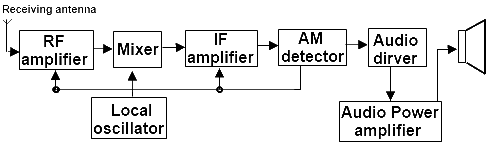
\includegraphics[width=.6\textwidth]{block}
	\end{center}
		\caption{Block Diagram}
		\label{fig:Block Diagram}
\end{figure}

\section{Section Name}
Lorem ipsum dolor sit amet, consectetur adipiscing elit. Curabitur non velit leo. Nullam dapibus libero condimentum tellus vehicula suscipit. Mauris non finibus augue. Nunc urna tellus, dapibus eu tellus ac, hendrerit pretium quam. Mauris dapibus nec ante nec iaculis. Mauris sodales felis sed neque volutpat venenatis. Morbi pellentesque sit amet dolor a rhoncus. Phasellus interdum augue quis dui vehicula malesuada. Quisque nisl dolor, ornare quis sodales vel, fermentum nec neque. 

\begin{enumerate}
\item First point.
\item Second point.
\end{enumerate}

\subsection{Subsection Name}
Lorem ipsum dolor sit amet, consectetur adipiscing elit. Curabitur non velit leo. Nullam dapibus libero condimentum tellus vehicula suscipit. Mauris non finibus augue. Nunc urna tellus, dapibus eu tellus ac, hendrerit pretium quam. Mauris dapibus nec ante nec iaculis. Mauris sodales felis sed neque volutpat venenatis. Morbi pellentesque sit amet dolor a rhoncus. Phasellus interdum augue quis dui vehicula malesuada. Quisque nisl dolor, ornare quis sodales vel, fermentum nec neque. 

\begin{itemize}
\item First point.
\item Second point.
\end{itemize}



\section{Algorithm/Tcolorbox}


\begin{tcolorbox}
\begin{tcolorbox}
\textsc{ALGORITHM:  An Image Authentication \& Reconstruction Scheme}
\end{tcolorbox}
\textbf{Require:} I\\
\textbf{Require:} h(), f (), g(), $ \mathrm{f^{-1}()} $, $ \mathrm{g^{-1}()} $\\
\textbf{Require:} b, B : b $ \leq $ B 

{$\;\;\;$}\hspace{1.cm} \textbf{for} i = 1 $ \rightarrow $ N do

Reconstruct $ I_i^, :e_i \neq 1  $ 
\end{tcolorbox}




\chapter{CIRCUIT DIAGRAM AND EXPLANATION}

\section{Circuit  Diagram}

\begin{figure}[H]
	\begin{center}
		\leavevmode
			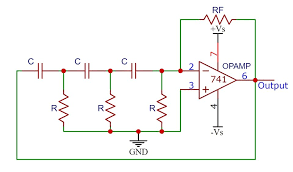
\includegraphics[width=.6\textwidth]{circuit}
	\end{center}
		\caption{Circuit Diagram}
		\label{fig:Circuit Diagram}
\end{figure}

\section{Section Name}
Lorem ipsum dolor sit amet, consectetur adipiscing elit. Curabitur non velit leo. Nullam dapibus libero condimentum tellus vehicula suscipit. Mauris non finibus augue. Nunc urna tellus, dapibus eu tellus ac, hendrerit pretium quam. Mauris dapibus nec ante nec iaculis. Mauris sodales felis sed neque volutpat venenatis. Morbi pellentesque sit amet dolor a rhoncus. Phasellus interdum augue quis dui vehicula malesuada. Quisque nisl dolor, ornare quis sodales vel, fermentum nec neque. 

\begin{enumerate}
\item First point.
\item Second point.
\end{enumerate}

\subsection{Subsection Name}
Lorem ipsum dolor sit amet, consectetur adipiscing elit. Curabitur non velit leo. Nullam dapibus libero condimentum tellus vehicula suscipit. Mauris non finibus augue. Nunc urna tellus, dapibus eu tellus ac, hendrerit pretium quam. Mauris dapibus nec ante nec iaculis. Mauris sodales felis sed neque volutpat venenatis. Morbi pellentesque sit amet dolor a rhoncus. Phasellus interdum augue quis dui vehicula malesuada. Quisque nisl dolor, ornare quis sodales vel, fermentum nec neque. 

\begin{itemize}
\item First point.
\item Second point.
\end{itemize}


\section{Sample Table 2}

\begin{table}[h]
\begin{center}
\begin{tabular}{|c|l|c|c|c|}
 \hline
   &                          &          &            &        \\ 
 \textbf{No} & \textbf{Particular} & \textbf{Quantity} & \textbf{Unit Price} & \textbf{Amount} \\ 
   &                          &          &            &        \\ \hline
1  & PIC 16F877A              & 1        & 150        & 150    \\ \hline
2  & Transformer              & 1        & 100        & 100    \\ \hline
\multicolumn{4}{|l}{\textbf{Total}}               \vline              & \textbf{1302} \\  \hline    
\end{tabular}
\end{center}
\captionof{table}{List of Devices}
\end{table}


\chapter{COMPONENTS USED}

 \section{Arduino Board}

\begin{figure}[H]
	\begin{center}
		\leavevmode
			\includegraphics[width=.6\textwidth]{arduino}
	\end{center}
		\caption{Arduino Board}
		\label{fig:Arduino Board}
\end{figure}

\section{Section Name}
Lorem ipsum dolor sit amet, consectetur adipiscing elit. Curabitur non velit leo. Nullam dapibus libero condimentum tellus vehicula suscipit. Mauris non finibus augue. Nunc urna tellus, dapibus eu tellus ac, hendrerit pretium quam. Mauris dapibus nec ante nec iaculis. Mauris sodales felis sed neque volutpat venenatis. Morbi pellentesque sit amet dolor a rhoncus. Phasellus interdum augue quis dui vehicula malesuada. Quisque nisl dolor, ornare quis sodales vel, fermentum nec neque. 

\begin{enumerate}
\item First point.
\item Second point.
\end{enumerate}

\subsection{Subsection Name}
Lorem ipsum dolor sit amet, consectetur adipiscing elit. Curabitur non velit leo. Nullam dapibus libero condimentum tellus vehicula suscipit. Mauris non finibus augue. Nunc urna tellus, dapibus eu tellus ac, hendrerit pretium quam. Mauris dapibus nec ante nec iaculis. Mauris sodales felis sed neque volutpat venenatis. Morbi pellentesque sit amet dolor a rhoncus. Phasellus interdum augue quis dui vehicula malesuada. Quisque nisl dolor, ornare quis sodales vel, fermentum nec neque. 

\begin{itemize}
\item First point.
\item Second point.
\end{itemize}


\begin{figure}
        \centering
        \begin{subfigure}[b]{0.3\textwidth}
                \includegraphics[width=\textwidth]{temp}
                \caption{Temperature Sensor}
                \label{fig:Temperature Sensor}
        \end{subfigure}%
        ~ %add desired spacing between images, e. g. ~, \quad, \qquad, \hfill etc.
          %(or a blank line to force the subfigure onto a new line)
        \begin{subfigure}[b]{0.3\textwidth}
                \includegraphics[width=\textwidth]{pressure}
                \caption{Pressure Sensor}
                \label{fig:Pressure Sensor}
        \end{subfigure}
        ~ %add desired spacing between images, e. g. ~, \quad, \qquad, \hfill etc.
          %(or a blank line to force the subfigure onto a new line)
        \begin{subfigure}[b]{0.3\textwidth}
                \includegraphics[width=\textwidth]{gassensor}
                \caption{Gas Sensor}
                \label{fig:Gas Sensor}
        \end{subfigure}
        \caption{Important Sensors}\label{fig:Main Sensors}
\end{figure}

\chapter{IMPLEMENTATION AND DESIGN}
\thispagestyle{empty}
Lorem ipsum dolor sit amet, consectetur adipiscing elit, sed do eiusmod tempor incididunt ut labore et dolore magna aliqua. Ut enim ad minim veniam, quis nostrud exercitation ullamco laboris nisi ut aliquip ex ea commodo consequat. Duis aute irure dolor in reprehenderit in voluptate velit esse cillum dolore eu fugiat nulla pariatur. Excepteur sint occaecat cupidatat non proident, sunt in culpa qui officia deserunt mollit anim id est laborum \nomenclature[Ch]{Ch}{Chapter} 


\section{PCB Layout / bread board set up details}
Lorem ipsum dolor sit amet, consectetur adipiscing elit, sed do eiusmod tempor incididunt ut labore et dolore magna aliqua. 

\begin{enumerate}
\item First point.
\item Second point.
\end{enumerate}

\section{Mechanical Design and Implementation}
Lorem ipsum dolor sit amet, consectetur adipiscing elit, sed do eiusmod tempor incididunt ut labore et dolore magna aliqua. 
\begin{itemize}
\item First point.
\item Second point.
\end{itemize}

\section{Details of Software used}
Lorem ipsum dolor sit amet, consectetur adipiscing elit, sed do eiusmod tempor incididunt ut labore et dolore magna aliqua. 

\begin{enumerate}
\item First point.
\item Second point.
\end{enumerate}

\subsection{Subsection Name}
Lorem ipsum dolor sit amet, consectetur adipiscing elit, sed do eiusmod tempor incididunt ut labore et dolore magna aliqua. 

\begin{itemize}
\item First point.
\item Second point.
\end{itemize}


\chapter{EXPLANATION OF CODE}


\section{Sample Table 3}

\begin{table}[h]
\begin{center}
\begin{tabular}{|c|l|c|c|c|}
 \hline
   &                          &          &            &        \\ 
 \textbf{No} & \textbf{Particular} & \textbf{Quantity} & \textbf{Unit Price} & \textbf{Amount} \\ 
   &                          &          &            &        \\ \hline
1  & PIC 16F877A              & 1        & 150        & 150    \\ \hline
2  & Transformer              & 1        & 100        & 100    \\ \hline
\multicolumn{4}{|l}{\textbf{Total}}               \vline              & \textbf{1302} \\  \hline    
\end{tabular}
\end{center}
\captionof{table}{List of Items}
\end{table}

\chapter{TESTING AND RESULTS}
\thispagestyle{empty}
Lorem ipsum dolor sit amet, consectetur adipiscing elit, sed do eiusmod tempor incididunt ut labore et dolore magna aliqua. \nomenclature[Ch]{Ch}{Chapter} 


\section{Testing Procedure}
Lorem ipsum dolor sit amet, consectetur adipiscing elit, sed do eiusmod tempor incididunt ut labore et dolore magna aliqua. 

\begin{enumerate}
\item First point.
\item Second point.
\end{enumerate}

\section{Observations and Output}
Lorem ipsum dolor sit amet, consectetur adipiscing elit, sed do eiusmod tempor incididunt ut labore et dolore magna aliqua. 

\begin{itemize}
\item First point.
\item Second point.
\end{itemize}

\section{Performance Analysis}
Lorem ipsum dolor sit amet, consectetur adipiscing elit, sed do eiusmod tempor incididunt ut labore et dolore magna aliqua. 

\begin{enumerate}
\item First point.
\item Second point.
\end{enumerate}

\subsection{Subsection Name}
Lorem ipsum dolor sit amet, consectetur adipiscing elit, sed do eiusmod tempor incididunt ut labore et dolore magna aliqua. 

\begin{itemize}
\item First point.
\item Second point.
\end{itemize}



\chapter{APPLICATIONS, LIMITATIONS AND FUTURE SCOPE}
\thispagestyle{empty}Lorem ipsum dolor sit amet, consectetur adipiscing elit, sed do eiusmod tempor incididunt ut labore et dolore magna aliqua.  \nomenclature[Ch]{Ch}{Chapter} 


\section{Applications}
Lorem ipsum dolor sit amet, consectetur adipiscing elit, sed do eiusmod tempor incididunt ut labore et dolore magna aliqua. 

\begin{enumerate}
\item First point.
\item Second point.
\end{enumerate}

\section{Limitations}
Lorem ipsum dolor sit amet, consectetur adipiscing elit, sed do eiusmod tempor incididunt ut labore et dolore magna aliqua. 

\begin{itemize}
\item First point.
\item Second point.
\end{itemize}

\section{Future Scope}
Lorem ipsum dolor sit amet, consectetur adipiscing elit, sed do eiusmod tempor incididunt ut labore et dolore magna aliqua. 

\begin{enumerate}
\item First point.
\item Second point.
\end{enumerate}

\subsection{Subsection Name}
Lorem ipsum dolor sit amet, consectetur adipiscing elit, sed do eiusmod tempor incididunt ut labore et dolore magna aliqua. 

\begin{itemize}
\item First point.
\item Second point.
\end{itemize}



\chapter{CONCLUSION}
\thispagestyle{empty}
Lorem ipsum dolor sit amet, consectetur adipiscing elit, sed do eiusmod tempor incididunt ut labore et dolore magna aliqua.\cite{JSM} \nomenclature[Ch]{Ch}{Chapter} 



\section{section Name}
Lorem ipsum dolor sit amet, consectetur adipiscing elit, sed do eiusmod tempor incididunt ut labore et dolore magna aliqua. \cite{HAR}

\begin{itemize}
\item First point.
\item Second point.
\end{itemize}


%Enter your references here manually and then cite in the document in the format:
%\newpage
%\begin{thebibliography}{ widest_entry}
%\bibitem[ label1]{ cite_key1} bibliographic entry
%\bibitem[ label2]{ cite_key2} bibliographic entry
. . .
%\end{thebibliography}
%\cite[page_number]{cite_key}
%\cite[45]{Azuela}
    \newpage
    \begin{thebibliography}{9}
    \bibitem{JSM} J. S. McLean,, \textit{"A Re-Examination of the Fundamental Limits on the Radiation Q of Electrically Small Antennas," }, IEEt: Trans. Antennas Propag., AP-44, May 1996, pp. 672-676.
\bibitem{HAR}R. F. Harrington,, \textit{"Effect of antenna size on gain, bandwidth, and efficiency,"  }, Research National Bureau of Standards-D. Radio Propagation, vol. 640, no. 1, Jan.-Feb. 1960.
    \end{thebibliography}

%\clearpage % or \cleardoublepage
\addcontentsline{toc}{chapter}{Bibliography}



\begin{appendices}
\chapter{Coding}
\lstinputlisting{expt01_p1.m}
\newpage
\lstinputlisting{expt01_p2.m}
\chapter{Project Estimate}
\section{Sample Table 4}

\begin{table}[h]
\begin{center}
\begin{tabular}{|c|l|c|c|c|}
 \hline
   &                          &          &            &        \\ 
 \textbf{No} & \textbf{Particular} & \textbf{Quantity} & \textbf{Unit Price} & \textbf{Amount} \\ 
   &                          &          &            &        \\ \hline
1  & PIC 16F877A              & 1        & 150        & 150    \\ \hline
2  & Transformer              & 1        & 100        & 100    \\ \hline
\multicolumn{4}{|l}{\textbf{Total}}               \vline              & \textbf{1302} \\  \hline    
\end{tabular}
\end{center}
\captionof{table}{Bill Of Materials}
\end{table}


\chapter{Datasheets}

\end{appendices}



\end{document}










